\scanpage{397}
I am interested above all in the induced homomorphism
\[
 (4)\qquad
 \diagram{\begin{tikzcd}[ampersand replacement=\&]
 \deleted{\unsure{\mathcal A}}\mathcal{M}_{\rho,\sigma}
 \arrow[r,"\Theta"] \& G\simeq\mathrm{Gl}(2)_S
 \end{tikzcd}}
\]
it is \unsure{obvious|obviously} an epimorphism, for its image contains
trivially $SG$, so it suffices to see
that the composite with
\[
 \diagram{\begin{tikzcd}[ampersand replacement=\&]
 G/SG\arrow[r,"\det","\sim"'] \& \mathbb G_m
 \end{tikzcd}}
\]
is an epimorphism, i.e. that the composite with $\det$ is one,
now this composite is also the homomorphism (again denoted $\chi$)
\[
 (5)\qquad
 \diagram{\begin{tikzcd}[ampersand replacement=\&,column sep=large]
 \mathcal{M}_{\rho,\sigma}
 \arrow[r,"\substack{\text{canonical}\\\text{projection}}"]
 \arrow[d,phantom,"\rotatebox{90}{$\simeq$}"]
 \& S\mathcal{G}_{\rho,\sigma}^{*\unsure{\flat|\sharp}}(0)
 \deleted{\unsure{\infty}}
 \arrow[r,"\text{multiplier}"] \& \mathbb G_m \\
 S\mathcal{G}_{\rho,\sigma}^{*\unsure{\flat|\sharp}}(0)\mathbin{.}SG
 \& (\alpha,\beta,\mu,\varepsilon)\arrow[r,mapsto] \& \mu
 \end{tikzcd}}
\]
which is an epimorphism --- in terms of
\[
 (6)\qquad
 \diagram{\begin{tikzcd}[ampersand replacement=\&]
 S\mathcal{G}_{\rho,\sigma}^{*\unsure{\flat|\sharp}}(0)
 \arrow[r,hook] \& \deleted{\unsure{\mathbb G_m}}T_0\times T_\rho\times N'_\sigma
 \end{tikzcd}}
\]
this will be
\[
 \diagram{\begin{tikzcd}[ampersand replacement=\&]
 (\uline{u},\uline{a},\uline{b})\arrow[r,mapsto] \& \det\uline{u}
 \end{tikzcd}},
\]
in terms of
\[
 (7)\qquad
 \diagram{\begin{tikzcd}[ampersand replacement=\&]
 S\mathcal{G}_{\rho,\sigma}^{*\unsure{\flat|\sharp}}(0)
 \arrow[r,hook] \& T_\rho\times N'_\sigma
 \end{tikzcd}}
\]
this will be
\[
 \diagram{\begin{tikzcd}[ampersand replacement=\&]
 (\uline{a},\uline{b})\arrow[r] \& \det\uline{b}
 \end{tikzcd}}
\]
(cf. \uline{VIII}, page 489 in particular (25)).

Let us define
\[
 (8)\qquad
 \mathcal{M}_{\rho,\sigma}^{+}\overset{\text{definition}}{=}
 \operatorname{Ker}\left(
 \diagram{\begin{tikzcd}[ampersand replacement=\&]
 \mathcal{M}_{\rho,\sigma}\arrow[r,"\chi"] \& \mathbb G_m
 \end{tikzcd}}\right),
\]
we shall thus have a homomorphism of exact sequences
\margin{396}

\scanpage{398}
\mspage{500}
\[
 (9)\qquad
 \diagram{\begin{tikzcd}[ampersand replacement=\&,column sep=large,row sep=large]
 1\arrow[r,dash] \& \mathcal M_{\rho,\sigma}^{+}\arrow[r,dash]\arrow[d]
 \& \mathcal M_{\rho,\sigma}\arrow[r]\arrow[d,"\Theta"]
 \& \mathbb G_m\arrow[r]\arrow[d,"\deleted{\unsure{\det}}"] \& 1\\
 1\arrow[r] \& \deleted{\unsure{SLG}}SG\arrow[r,hook]
 \& G\arrow[r,"\det"] \& \mathbb G_m\arrow[r] \& 1
 \end{tikzcd}}
\]
which we shall compare with §39 page 299 (1)

As $\mathcal M_{\rho,\sigma}$ is flat of relative dimension
6, and $G$ \unsure{idem|idem} of relative dimension 4, the
kernel of the epimorphism $\Theta\colon\mathcal M_{\rho,\sigma}\longrightarrow G$ is
necessarily flat of relative dimension 2. \unsure{Let us denote} it by
$I_{\rho,\sigma}$, it is contained in the
kernel $J_{\rho,\sigma}$ (of relative dimension 3)
of the composite
\[
 \diagram{\begin{tikzcd}[ampersand replacement=\&]
 \mathcal M_{\rho,\sigma}\arrow[r]\&G\arrow[r]\&PG
 \end{tikzcd}},
\]
so that we have
\[
 (10)\qquad
 \diagram{\begin{tikzcd}[ampersand replacement=\&]
 1\arrow[r,dash]\&I_{\rho,\sigma}\arrow[r]\&J_{\rho,\sigma}\arrow[r]
 \&\mathbb G_m\arrow[r]\&1\arrow[r,dash]\&\unsure{1}
 \end{tikzcd}}
\]
and a composition series of $\mathcal M_{\rho,\sigma}$
\[
 (11)\qquad
 \diagram{\begin{tikzcd}[ampersand replacement=\&,column sep=large,row sep=large]
 1\arrow[r,phantom,"\subset"]
 \& I_{\rho,\sigma}\arrow[r,phantom,"\subset"]
 \arrow[rr,dash,start anchor=south,end anchor=south,
 to path={-- ++(0,-1.1) -- node[below] {$G$} ([yshift=-1.1cm]\tikztotarget) -- (\tikztotarget)}]
 \& J_{\rho,\sigma}\arrow[r,phantom,"\subset"]
 \arrow[r,dash,start anchor=south,end anchor=south,
 to path={-- ++(0,-0.4) -- node[below] {$PG\simeq SG/\mu_2$} ([yshift=-0.4cm]\tikztotarget) -- (\tikztotarget)}]
 \&\mathcal M_{\rho,\sigma}
 \end{tikzcd}}
\]
The group $J_{\rho,\sigma}$ plays the role of a
\uline{radical} --- we expect it to be commutative,
(of relative dimension 3) --- and \inserted{with components}
\unsure{toric|toric} if
\margin{397}

\scanpage{399}
$T_\rho^{\circ},T_\sigma^{\circ}$ are tori.

But I see that I am making
life complicated for myself by being too learned in my
\unsure{deductions|directions}. Indeed, by construction
of the $\frac12$ direct product, we have
\[
 \diagram{\begin{tikzcd}[ampersand replacement=\&,column sep=small,row sep=small]
 \mathcal M_{\rho,\sigma}=S\mathcal G_{\rho,\sigma}^{*}\mathbin{.}SG
 \arrow[r,hook,dash] \&(T_0\times T_\rho\times N'_\sigma)\mathbin{.}SG
 \arrow[d,phantom,"\rotatebox{90}{$\simeq$}"]\\
 \& (T_\rho\times N'_\sigma)\times\underbrace{(T_0\mathbin{.}SG)}_{G}
 \end{tikzcd}}
\]
thus
\[
 (12)\qquad
 \diagram{\begin{tikzcd}[ampersand replacement=\&,column sep=large,row sep=large]
 \mathcal M_{\rho,\sigma}\arrow[r,hook]\arrow[dr,"\Theta"']
 \&T_\rho\times N'_\sigma\times G\arrow[d,"\mathrm{pr}_3"]\\
 \&G
 \end{tikzcd}}
\]
moreover $\mathcal M_{\rho,\sigma}$ is defined in this
product by the conditions
\[
 (13)\qquad
 \begin{aligned}
 \mathcal M_{\rho,\sigma}&\subset T_\rho\times N'_\sigma\times G\\
 &=\{(x,y,f)\mid\det f=\det y=\varepsilon'\det x,\quad
 \varepsilon'^2=1\}
 \end{aligned}
\]
This shows that
\[
 (14)\qquad
 \begin{aligned}
 \unsure{I|J}_{\rho,\sigma}
 &\hookrightarrow T_\rho\times N'_\sigma\times\mathbb G_m\\
 &\simeq\{(x,y,\lambda)\mid
 \det\deleted{\unsure{x}}y=\deleted{\det}\varepsilon\det x=\lambda^2,
 \quad\varepsilon^2=1\}\\[1em]
 \unsure{J|I}_{\rho,\unsure{\sigma|x}}
 &\subset T_\rho\times N_\sigma^{\prime\unsure{\flat|\sharp}}\\
 &\simeq\{(x,y)\mid\det y=1,\ (\det x)^2=1\}
 \end{aligned}
\]
It seems more natural to me to
do the \unsure{dévissage} of $\mathcal M_{\rho,\sigma}$ starting
by going down to the identity component $\mathcal M_{\rho,\sigma}^{\circ}$,
\margin{398}

\scanpage{400}
\mspage{501}
the group
\[
 (15)\qquad
 \diagram{\begin{tikzcd}[ampersand replacement=\&,column sep=small,row sep=tiny]
 \inserted{\text{\unsure{component} of the identity}}\arrow[d,dash]\!\&\\[-0.3em]
 \mathcal M_{\rho,\sigma}/\mathcal M_{\rho,\sigma}^{\circ}
 \arrow[r,phantom,"\simeq"]
 \&\mathcal G_{\rho,\sigma}^{*}(0)/\mathcal G_{\rho,\sigma}^{*}(0)^{\circ}
 \simeq\mu_2\times\mu_2
 \end{tikzcd}}
\]
(cf. page 489 (23)), we shall thus have
\[
 \diagram{\begin{tikzcd}[ampersand replacement=\&,column sep=small,row sep=small]
 \mathcal M_{\rho,\sigma}^{\circ}=\mathcal G_{\rho,\sigma}^{*}(0)^{\circ}\mathbin{.}SG
 \arrow[r,hook,dash]
 \&(T_0\times T_\rho\times T_\sigma)\mathbin{.}SG
 \arrow[d,phantom,"\rotatebox{90}{$\simeq$}"]\\
 \&T_\rho\times T_\sigma\times
 \underbrace{(T_0\mathbin{.}SG)}_{\substack{\simeq\\G}}
 \arrow[d,phantom,"\rotatebox{90}{$\simeq$}"]\\
 \&T_\rho\times T_{\unsure{\sigma|\rho}}\times G
 \end{tikzcd}}
\]
\[
 (16)\qquad
 \begin{aligned}
 \mathcal M_{\rho,\sigma}^{\circ}&\lhook\joinrel\longrightarrow
 T_\rho\times T_\sigma\times G\\
 &\simeq\left\{
 \left(\underset{\substack{\rotatebox{90}{$\in$}\\\Gamma T_\rho}}{x},
 \underset{\substack{\rotatebox{90}{$\in$}\\\Gamma T_\sigma}}{y},
 \underset{\substack{\rotatebox{90}{$\in$}\\\Gamma G}}{f}\right)
 \mathrel{\Big|}\det x=\det y=\det f\right\}
 \end{aligned}
\]
Thus the kernel
\[
 (17)\qquad\left\{
 \begin{aligned}
 J_{\rho,\sigma}^{\circ}&\overset{\text{definition}}{=}
 \operatorname{Ker}\left(
 \diagram{\begin{tikzcd}[ampersand replacement=\&,row sep=tiny]
 \mathcal M_{\rho,\sigma}^{\circ}\arrow[r]\&PG
 \arrow[d,phantom,"\rotatebox{90}{$\simeq$}"]\\
 \&G/\mathbb G_m
 \end{tikzcd}}\right)\\
 &\simeq\left\{
 \left(\underset{\substack{\rotatebox{90}{$\in$}\\\Gamma T_\rho}}{x},
 \underset{\substack{\rotatebox{90}{$\in$}\\\Gamma T_\sigma}}{y},
 \underset{\substack{\rotatebox{90}{$\in$}\\\Gamma\mathbb G_m}}{\lambda}\right)
 \mathrel{\Big|}\det x=\det y=\unsure{\lambda^2}\right\}
 \deleted{\unsure{\simeq T_\rho\times_{\mathbb G_m}T_\sigma}}\\[0.6em]
 &\simeq T_\rho\times_{\mathbb G_m}T_\sigma
 =\{(x,y)\mid\det x=\det y\}\\
 &\simeq S\mathcal G_{\rho,\sigma}^{\unsure{*}}(0)^{\circ}
 \end{aligned}\right.
\]
Finally, we deduce from this that
\[
 (18)\qquad
 \begin{aligned}
 I_{\rho,\sigma}^{\circ}&\overset{\text{definition}}{=}
 \operatorname{Ker}\left(
 \diagram{\begin{tikzcd}[ampersand replacement=\&]
 \mathcal M_{\rho,\sigma}^{\circ}\arrow[r]\&G
 \end{tikzcd}}\right)\\
 &\simeq ST_\rho\times ST_\sigma
 =\left\{\left(
 \underset{\substack{\rotatebox{90}{$\in$}\\\Gamma T_\rho}}{x},
 \underset{\substack{\rotatebox{90}{$\in$}\\\Gamma T_\sigma}}{y}
 \right)\mathrel{\Big|}\det x=\det y=1\right\}.
 \end{aligned}
\]
Let us recapitulate:
\margin{399}

\scanpage{401}
\uline{Theorem} The group
\[
 (19)\qquad
 \diagram{\begin{tikzcd}[ampersand replacement=\&,column sep=small,row sep=small]
 \mathcal M_{\rho,\sigma}\arrow[r,phantom,"{\overset{\text{definition}}{\simeq}}"]
 \&\mathcal G_{\rho,\sigma}^{*}(0)\mathbin{.}SG
 \arrow[d,phantom,"\rotatebox{90}{$\subset$}"]
 \&\inserted{\text{cf. definition page 487' (20)}}\arrow[l]\\
 \&T_0\times T_\rho\times N'_\sigma\&
 \end{tikzcd}}
\]
is an extension of $\mu_2\times\mu_2$ by $\mathcal M_{\rho,\sigma}^{\circ}$
\[
 (20)\qquad
 \diagram{\begin{tikzcd}[ampersand replacement=\&]
 1\arrow[r]\&\mathcal M_{\rho,\sigma}^{\circ}\arrow[r,dash]
 \&\mathcal M_{\rho,\sigma}\arrow[r]\&\mu_2\times\mu_2\arrow[r]\&1
 \end{tikzcd}}.
\]
\inserted{deduced from
\[
 \diagram{\begin{tikzcd}[ampersand replacement=\&]
 \mathcal G_{\rho,\sigma}^{*}\deleted{\unsure{(0)}}\arrow[r]\&\mu_2\times\mu_2\\
 \deleted{(\alpha,\beta,\mu,\varepsilon)}\ (\alpha,\beta,\mu,\varepsilon)
 \arrow[r]\&(\det\alpha,\varepsilon(=\det\uline b))
 \end{tikzcd}}
\]}
In $\mathcal M_{\rho,\sigma}^{\circ}$ \unsure{we}
\deleted{\unsure{have two}}\inserted{the} subgroup
\deleted{noteworthy: the subgroup} \uline{central}
(in the whole of $\mathcal M_{\rho,\sigma}$)
\[
 (21)\qquad
 \diagram{\begin{tikzcd}[ampersand replacement=\&]
 ST_\rho\times ST_\sigma\arrow[r,hook]
 \&\mathcal G_{\rho,\sigma}^{*}(0)\arrow[r,hook]
 \&\mathcal M_{\rho,\sigma}
 \end{tikzcd}},
\]
and \unsure{we have} an exact sequence
\[
 \deleted{\unsure{(22)}}\quad\unsure{(21)|(22)}\qquad
 \diagram{\begin{tikzcd}[ampersand replacement=\&,row sep=large]
 1\arrow[r]\arrow[rrrr,dash,start anchor=north west,end anchor=south east,
 to path={([xshift=-3mm,yshift=5mm]\tikztostart) rectangle
 ([xshift=3mm,yshift=-5mm]\tikztotarget)}]
 \&ST_\rho\times ST_\sigma\arrow[r]\&\mathcal M_{\rho,\sigma}^{\circ}
 \arrow[r,"\Theta"]\&G\arrow[r]\&1\\
 \&\&\inserted{SG}\arrow[u,hook]\&\&
 \end{tikzcd}}
\]
We have \deleted{\unsure{therefore}} in $\mathcal M_{\rho,\sigma}^{\circ}$
a \deleted{composition series}\inserted{structure of an \unsure{extension}}
\[
 \diagram{\begin{tikzcd}[ampersand replacement=\&,row sep=large]
 \text{\unsure{read}}\ \deleted{1\subset ST_\rho\times ST_\sigma\times SG
 \subset J_{\rho,\sigma}^{\circ}\unsure{\times|\mathbin{.}}SG}\\
 \inserted{\begin{gathered}
 \text{\uline{NB}}\\
 J_{\rho,\sigma}^{\circ}\text{ is also}\\
 \text{central in }\mathcal M_{\rho,\sigma}\\
 \text{and }J_{\rho,\sigma}^{\circ}\cap SG\simeq
 \end{gathered}}
 \arrow[u,bend left=15]\arrow[u,bend right=20]
 \end{tikzcd}}
\]
\[
 (23)\qquad
 \diagram{\begin{tikzcd}[ampersand replacement=\&,row sep=small]
 \&\&x\arrow[r,mapsto]\&\chi(x),\varepsilon(x),\varepsilon'(x)\&\\
 1\arrow[r]\arrow[rrrr,dash,start anchor=north west,end anchor=south east,
 to path={([xshift=-3mm,yshift=5mm]\tikztostart) rectangle
 ([xshift=3mm,yshift=-5mm]\tikztotarget)}]
 \&ST_\rho\times ST_\sigma\times SG\arrow[r]
 \&\mathcal M_{\rho,\sigma}\arrow[r]\&\mathbb G_m\times\mu_2\times\mu_2\arrow[r]\&1
 \end{tikzcd}}
\]
i.e.
\[
 (24)\qquad
 \mathcal M_{\rho,\sigma}^{\circ+}\simeq ST_\rho\times ST_\sigma\times SG\unsure{,|\}}
\]
\deleted{and we also have (\unsure{using} the inclusion
$(G\longrightarrow\mathcal M_{\rho,\sigma}^{\circ})$)}
\inserted{\unsure{nonexistent}}
\[
 \diagram{\begin{tikzcd}[ampersand replacement=\&,nodes in empty cells]
 \deleted{ST_\rho\times ST_\sigma\times G}
 \arrow[r,"\deleted{\unsure{\longrightarrow}}",phantom]
 \&\deleted{\mathcal M_{\rho,\sigma}^{\circ}}
 \arrow[r,"\deleted{\longrightarrow}",phantom]\&\deleted{1}
 \end{tikzcd}}
\]
We have a canonical homomorphism
\[
 (25)\qquad
 \diagram{\begin{tikzcd}[ampersand replacement=\&,column sep=small,row sep=small]
 \mu_2\times\mu_2\times\mu_2\arrow[r,hook]
 \&\mathcal M_{\rho,\sigma}^{\circ+}
 \overset{\text{definition}}{=}\operatorname{Ker}
 (\mathcal M_{\rho,\sigma}^{\circ}\overset{\chi}{\longrightarrow}\mathbb G_m)
 \arrow[d,phantom,"{\rotatebox{90}{$\simeq$}\ (24)}"]\\
 \&ST_\rho\times ST_\sigma\times SG
 \end{tikzcd}}
\]
\margin{400}

\scanpage{402}
\mspage{502}

thanks to the canonical inclusions
\[
\tag{26}
\mu_2\hookrightarrow ST_\rho,\qquad
\mu_2\hookrightarrow ST_\sigma,\qquad
\mu_2\hookrightarrow SG
\]
giving rise to canonical homomorphisms already \unsure{considered} elsewhere
\[
\tag{27}
\Sigma=(\mathbb Z/2\mathbb Z)^3\longrightarrow
\Gamma\mathcal M_{\rho,\sigma}^{\circ+}\deleted{\unsure{+}}
\subset\Gamma\mathcal M_{\rho,\sigma}^{\unsure{+|*}}.
\]

I am going to introduce for the group $\mathcal M_{\rho,\sigma}$ notations which paraphrase the notations $\mathcal M_{0,3}$ etc., in the context of group schemes. The invariant subgroup $SG$ of $\mathcal M_{\rho,\sigma}$ will also be denoted $\widetilde G_{\rho,\sigma}^{+}$ (the analogue of $\widehat{\widetilde G}_{0,3}^{+}$), the quotient
\[
\tag{28}
\deleted{\unsure{\mathcal M}}
\mathcal M_{\rho,\sigma}/\widetilde G_{\rho,\sigma}^{+}
\simeq\tau_{\rho,\sigma}^{!}
\]
\unsure{paraphrases} $\tau_{0,3}^{!}$, we have moreover
\[
\tag{29}
\tau_{\rho,\sigma}^{!}\simeq S\mathcal G_{\rho,\sigma}^{*}(0)
\hookrightarrow T_0\times T_\rho\times N'_\sigma
\]
\margin{\unsure{Seen hanging around a bit} the sign $!$, (\unsure{which} \unsure{has fallen from the sky} --- \unsure{even in the section following the} \uline{\unsure{X}}) it is $\Gamma_{\rho,\sigma}$ (and not $\tau_{\rho,\sigma}$ \unsure{without the exponent} !) that one ought to \unsure{denote} this group by !}

--- in what follows the simpler and more suggestive notation $\tau_{\rho,\sigma}$ will be used in preference to $S\mathcal G_{\rho,\sigma}^{*}(0)$. We thus have
\[
\tag{30}
\diagram{\begin{tikzcd}[ampersand replacement=\&,column sep=small]
1\arrow[r]\&\widetilde G_{\rho,\sigma}^{+}\arrow[r]\arrow[d,phantom,"\rotatebox{90}{$\simeq$}"]\&\mathcal M_{\rho,\sigma}\arrow[r]\&\tau_{\rho,\sigma}^{!}\arrow[r]\&1\\
\&SG\simeq\mathrm{Sl}(2)_S\&\&\&
\end{tikzcd}}
\]
and a canonical splitting as a semidirect product
\[
\tag{31}
\mathcal M_{\rho,\sigma}\simeq\mathcal M_{\rho,\sigma}(0)\mathbin{.}\widetilde G_{\rho,\sigma}^{+}
\]
\margin{401}

\scanpage{403}

where
\[
\tag{32}
\diagram{\begin{tikzcd}[ampersand replacement=\&]
\mathcal M_{\rho,\sigma}(0)\arrow[r,hook]\arrow[dr,"\sim"']\&\mathcal M_{\rho,\sigma}\arrow[d,"\mathrm{can}"]\\
\&\tau_{\rho,\sigma}^{!}
\end{tikzcd}}
\]
is a subgroup isomorphic to $\tau_{\rho,\sigma}^{!}$ --- which corresponds to the subgroup $\mathcal M_{0,3}^{!\sim}(0)$ in $\mathcal M_{0,3}^{\sim}$ ($\S46$, $\uline{\mathrm V}$).

\uline{Remark.} One would like to introduce a $\tau_{\rho,\sigma}$ extension \inserted{(or product)} of $\tau_{\rho,\sigma}^{!}$ by a group such as $\widetilde G_3$ (which would be denoted $\tau_{\rho,\sigma}^{+}$), in relation to a subgroup $\pi_{\rho,\sigma}$ of $\widetilde G_{\rho,\sigma}^{+}$ \deleted{which} such that $\widetilde G_{\rho,\sigma}^{+}/\pi_{\rho,\sigma}\simeq\widetilde G_3$ --- but this is not possible in the context of group \uline{schemes} (even in the modular special case), since $\widetilde G_{\rho,\sigma}^{+}\simeq\mathrm{Sl}(2)_S$ is \deleted{\illegible{1}} \unsure{relatively} connected over $S$. On the other hand one can, in the ``modular case'' $\rho=\begin{pmatrix}0&1\\-1&1\end{pmatrix}$, $\sigma=\begin{pmatrix}0&1\\-1&0\end{pmatrix}$ introduce a canonical section
\[
\tag{33}
\unsure{\dot\tau|\dot t}=\unsure{\dot\tau_\infty|\dot t_\infty}\in\Gamma(\tau_{\rho,\sigma}^{!})
\]
whose representative $\tau_\infty$ in $\Gamma\unsure{\mathcal M}_{\rho,\sigma}^{!}(0)$ is explicitly given as
\[
\tag{34}
\tau_\infty=\begin{pmatrix}-1&0\\0&+1\end{pmatrix}.
\]

(It would be interesting to see whether, outside the
\margin{402}

\scanpage{404}
\mspage{503}

modular case, one can introduce ``anti-involutions'' which generalize the geometric reflections
\[
\tag{35}
\left\{
\begin{aligned}
\deleted{\unsure{\tau}}r_0&=\tau'_\infty=\begin{pmatrix}0&1\\1&\unsure{0}\end{pmatrix}\\
r_1&=-\tau'_0=\begin{pmatrix}-1&1\\0&1\end{pmatrix}\\
r_\infty&=\tau_\infty=\begin{pmatrix}-1&0\\0&+1\end{pmatrix}
\end{aligned}
\right.
\qquad\text{(cf. p. $335'$, $\S42$, $\uline{\mathrm{IV}}$)}
\]
I am convinced that one can. Besides, had we not brought to light in $\mathcal M_{\rho,\sigma}$ a subgroup $\mu_2\times\mu_2\times\mu_2$, \deleted{\unsure{corresponding} \unsure{in}} \inserted{giving} the three remarkable sections (corresponding respective\textsuperscript{ly} to the \deleted{three} sections $-1$ of the three factors $\mu_2$)? But I am getting things mixed up here --- these sections were sections of $\mathcal M_{\rho,\sigma}^{\circ}$ --- whereas the sections \deleted{\unsure{modular}} \inserted{$\tau_\infty,\tau'_\infty,\tau'_0$} \inserted{are of} multiplier
\deleted{in fact the center of $\mathcal M_{\rho,\sigma}$ is \unsure{isomorphic to}}
\inserted{\uline{$Z_{\rho,\sigma}\overset{\mathrm{df}}=(\mathrm{Centr}\,\mathcal M_{\rho,\sigma}^{\circ})$}.}
$-1$, thus correspond to $\varepsilon=\varepsilon'=-1$, thus correspond to the ``least trivial'' section \inserted{$(-1,-1)$} of $\mathcal M_{\rho,\sigma}/\mathcal M_{\rho,\sigma}^{\circ}=\mu_2\times\mu_2$.

\deleted{Let us then return to}
\[
\deleted{(36)}\qquad
\diagram{\begin{tikzcd}[ampersand replacement=\&,column sep=small,nodes in empty cells]
\deleted{\tau_{\rho,\sigma}^{!}\simeq\mathcal G_{\rho,\sigma}^{*}(0)}\arrow[r,hook]\arrow[d,phantom,"\deleted{\rotatebox{90}{$\simeq$}}"]\&\deleted{T_0\times T_\rho\times N'_\sigma}\\
\deleted{\left\{\{u,\underline a,\underline b\}\mid\det\underline u=\det\underline b=\varepsilon'\det\underline a,\ {\varepsilon'}^2=1\right\}}\&
\end{tikzcd}}
\]
\deleted{and let us recall that we have}
\[
\diagram{\begin{tikzcd}[ampersand replacement=\&,nodes in empty cells]
\deleted{T_0}\arrow[r,"\deleted{\sim}"',"\deleted{\delta_0:\ u\mapsto\det u}"]\&\deleted{\mathbb G_m}
\end{tikzcd}}
\]
\deleted{and canonical \unsure{``injective''} homomorphisms}
\[
\diagram{\begin{tikzcd}[ampersand replacement=\&,nodes in empty cells]
\deleted{\mathbb G_m}\arrow[r,"\deleted{j_\rho}"]\&\deleted{T_\rho}\\
\deleted{\mathbb G_m}\arrow[r,"\deleted{j_\sigma}"]\&\deleted{T_\sigma}
\end{tikzcd}}
\]
\deleted{whose \unsure{composite} with $\delta_\rho,\delta_\sigma$ (the determinant homomorphisms) are $\lambda\longrightarrow\lambda^2$. Thus in the second \unsure{side} of $(36)$ there is a}
\margin{403}

\scanpage{405}
\deleted{subgroup of \unsure{trivial centrality}}
\deleted{$\unsure{\mathbb G_m\times}$}
\[
\diagram{\begin{tikzcd}[ampersand replacement=\&,nodes in empty cells]
\deleted{\mathbb G_m\times\mathbb G_m\times\mathbb G_m}\arrow[r,hook]\&\deleted{T_0\times\unsure{T_\rho}\times N'_\sigma}
\end{tikzcd}}
\]

Let us do the calculations to determine the invariants $\alpha\ \beta\ \ldots$ corresponding to $r_0,r_1,r_\infty$.

i) $\displaystyle r_\infty=\tau_\infty=\begin{pmatrix}-1&0\\0&1\end{pmatrix}\in\mathrm{Gl}(2,\mathbb Z)\subset\mathrm{Gl}(2,\widehat{\mathbb Z})^{\pm1}$

We even have: $\tau_\infty\in\unsure{T'_0|B'_0}(\mathbb Z)$, \deleted{so it corresponds to} \inserted{it is the only element} \deleted{$(\alpha,\beta,f)$ with $f=1$,} that is nontrivial in $T'_0(\mathbb Z)\simeq\mathbb G_m(\mathbb Z)\simeq\{\pm1\}$. \deleted{\unsure{The}}

The inner automorphism it defines in $\Pi_{0,3}$ or in $\mathrm{Sl}(2,\mathbb Z)$ --- or their profinite completions --- stabilizes the subgroup $\widetilde L_0$ generated by $\varepsilon_0$ \inserted{(\unsure{i.e.} $L_0$ generated by $\varepsilon_0^2=\ell_0$)}
\[
\tau_\infty(\varepsilon_0)=\varepsilon_0^{-1},\qquad\tau_\infty(\ell_0)=\ell_0^{-1}
\]
$\unsure{(\ast)}$

thus
\[
\tau_\infty\in\mathcal M_{0,3}^{!\sim}[0]
\]
\deleted{\unsure{etc.}} \deleted{\unsure{we find}} it is of the form $u_{\alpha,\beta}$, \deleted{\unsure{we}} the calculations already done give
\[
\alpha=\tau_\infty,\qquad
\unsure{\zeta|\xi}=g=\alpha\rho(\alpha)^{-1}=-\ell_1^{-1}
=-\begin{pmatrix}1&0\\-2&1\end{pmatrix}
\]
(watch the sign $-$ when doing the calculations in $\mathrm{Sl}(2,\mathbb Z)$ and not in $\mathrm{Sl}(2,\mathbb Z)'$ !)
\[
\begin{aligned}
\beta&=\underline1,\qquad\eta=h=1,\\
\mu&=-1,\qquad\varepsilon=\varepsilon_2(\mu)=-1,\qquad
\varepsilon'=\unsure{\varepsilon_3(\mu)|\varepsilon_3^b(\mu)}=-1.
\end{aligned}
\]

we have here $B=0,D=-1$, thus
\[
u=\begin{pmatrix}
\deleted{\unsure{\mu}}\frac1D=\mu&\frac BD=\unsure{\mu D|\mu B}\\
0&1
\end{pmatrix}
=\begin{pmatrix}-1&0\\0&1\end{pmatrix}=\tau_\infty
\]
\[
\underline a=\alpha^{-1}u=\tau_\infty^{-1}\tau_\infty=\underline1,
\qquad\underline b=\beta^{-1}u=\tau_\infty.
\]
thus
\[
\tag{36}
r_\infty=\tau_\infty=
\deleted{\unsure{(\underline u_\infty=-1,\underline a_\infty=1,\underline b_\infty=\tau_\infty)}}
\inserted{(\underline u_\infty=\tau_\infty,\underline a_\infty=1,\underline b_\infty=\tau_\infty)}
\in T_0\times T_\rho\times N'_\sigma.
\]
\inserted{the nontrivial element of ${}_2T_0(\mathbb Z)\simeq{}_2T'_0(\mathbb Z)$}

\uline{N.B.} Let more generally
\[
\underline u=\begin{pmatrix}\mu&\lambda\\0&1\end{pmatrix}
\in\deleted{\unsure{\mathrm{Gl}}}\,B'_0(\widehat{\mathbb Z})\subset\mathrm{Gl}(2,\mathbb Z)
\]
and let us consider the \deleted{inner} automorphism of $\mathrm{Sl}(2,\mathbb Z)'\unsure{\simeq}$ which it induces, hence an automorphism \inserted{($\in\mathcal M_{0,3}^{!\sim}$)} of $\widehat{\widetilde G}_{0,3}^{+}$, what are these invariants $\alpha,\beta$ etc.? We shall be able obvious-
\margin{404}

\scanpage{406}
\mspage{504}
ly take $f=1$, and we will have
\[
\alpha=\underline u,\qquad\text{whence}\qquad\underline a=1,
\]
on the other hand, let us note that $\mu\in\{\pm1\}\inserted{\text{i.e. }\mu}=(-1)^k$ $(k\in\mathbb Z/2\mathbb Z)$, we will have $\varepsilon=\varepsilon'=\mu$, and if $\mu=1$ \inserted{(i.e. $u\in\mathrm{Sl}(2,\mathbb Z)$)} we will have $\beta=\underline u$ (\deleted{since} hence $\underline b=1$, otherwise $\beta=\deleted{\unsure{\tau_\infty}}u\tau_\infty$ hence $\underline b=\tau_\infty$), in all cases we will have
\[
\beta=u\tau_\infty^k,\qquad\underline b=\tau_\infty^k,
\]
in summary
\[
\tag{37}
\begin{gathered}
\underline u=\left(
\underset{\substack{\rotatebox{90}{$\in$}\\\Gamma B'_0}}{\underline u=u},
\underset{\substack{\rotatebox{90}{$\in$}\\\Gamma T_\rho}}{\underline a=1},
\underset{\substack{\rotatebox{90}{$\in$}\\\Gamma N'_\sigma}}{\underline b=\tau_\infty^k}
\right)
\in
\underset{\substack{\rotatebox{90}{$=$}\\\inserted{\mathcal M_{\rho,\sigma}[0](\widehat{\mathbb Z})}}}
{\deleted{\unsure{\mathcal M}}\,\unsure{S\mathcal G|\mathcal G}_{\rho,\sigma}^{*}(\unsure{0})(\widehat{\mathbb Z})}
\subset\left(B'_0\times T_\rho\times N'_\sigma\right)(\widehat{\mathbb Z}).
\end{gathered}
\]

\deleted{$2^\circ)$ $r_1=-\tau'_0=\begin{pmatrix}-1&1\\0&1\end{pmatrix}$. To it we can \unsure{apply the}}

But this is not an element in \deleted{\unsure{preceding paragraph|preceding argument}} \unsure{normalized} form --- \deleted{besides \unsure{we}} \inserted{i.e.} it is not in $\Gamma\mathcal G_{\rho,\sigma}^{*}(0)$, unless $\lambda=0$. \deleted{\unsure{We will have}}

$2^\circ)$ $r_1=-\tau'_0=\begin{pmatrix}-1&1\\0&1\end{pmatrix}$, this is precisely a case that falls under \unsure{the preceding remarks}, we will have
\[
\tag{38}
\unsure{r_1|\tau_1}=-\tau'_0=
\left(\underline u_1=-\tau'_0=\begin{pmatrix}-1&1\\0&1\end{pmatrix},\ \underline a=1,\ \underline b=\tau_\infty\right)
\in\mathcal M_{\rho,\sigma}[0](\mathbb Z)
\]
\margin{\uline{N.B.} \unsure{reducing} modulo $L_0\subset\widetilde G_{\rho,\sigma}^{+}$, $\tau_\infty$ and $r_1$ have the same image in $\tau_{\rho,\sigma}$, namely $(-1,1,\tau_\infty)$.}

$3^\circ)$ $r_0=\tau'_\infty=\begin{pmatrix}0&1\\1&0\end{pmatrix}$, this time we have an automorphism \inserted{of $\widetilde G_{0,3}^{+}$ \unsure{or} $\widetilde G_{0,3}^{+\wedge}$} which does not normalize $L_0$ --- that is better, if we want $r_0,r_1,r_\infty$ to generate $\mathrm{Gl}(2,\mathbb Z)$ (or even ``only'' $\mathrm{Gl}(2,\mathbb Z)'$) !

We have $\tau'_\infty=\tau_\infty\sigma_\infty$, so its image in $\mathcal M_{\rho,\sigma}(\mathbb Z)\subset\mathcal M_{\rho,\sigma}(\widehat{\mathbb Z})$ is \deleted{\unsure{like}} the product of the images of $\tau_\infty$ and $\sigma_\infty$ --- the first was computed in $1^\circ$, the second is tautological since $SG\simeq\widetilde G_{\rho,\sigma}^{+}$ and $\sigma_\infty\in SG(\mathbb Z)$. We will note that \deleted{$\unsure{\tau'_\infty}$} $r_0=\tau'_\infty$ thus has the same image
\margin{405}

\scanpage{407}
\mspage{\unsure{504}}

in $\tau_{\rho,\sigma}(\mathbb Z)$ as $r_\infty=\tau_\infty$ and $r_1=-\tau'_0$, it is always the same element \deleted{\illegible{1}}
\[
(39)\qquad (-1,1,\tau_\infty)\in
\left(\underset{\substack{\wr\\\mathbb G_m}}{T_0}\times T_\rho\times N'_\sigma\right)(\mathbb Z)
\]

Let us moreover compute
\[
T_0\times T_\rho\times N'_\sigma(\mathbb Z)
=T_0(\mathbb Z)\times T_\rho(\mathbb Z)\times N'_\sigma(\mathbb Z)
\]
We have
\[
(40)\quad
\left\{
\begin{array}{ll}
T_0\simeq\mathbb G_m,\quad T_0(\mathbb Z)\simeq\{\pm1\}&\\[2pt]
T_\rho(\mathbb Z)\simeq(\mathbb Z+\mathbb Z.\rho)^*\simeq\mathbb Z/6\mathbb Z
&\begin{array}{l}\text{group generated}\\\text{by }\rho\end{array}\\[2pt]
N'_\sigma(\mathbb Z)\simeq\{1,\tau_\infty\}.T_\sigma(\mathbb Z)
&\text{(semidirect product)}\\[2pt]
T_\sigma(\mathbb Z)\simeq(\mathbb Z+\mathbb Z\sigma)^*\simeq\mathbb Z/4\mathbb Z
&\begin{array}{l}\text{group generated}\\\text{by }\sigma\end{array}\\[2pt]
N'_\sigma(\mathbb Z)\simeq D_4
&\begin{array}{l}\text{\unsure{dihedral} group of order \unsure{4}}\\\text{(``symmetries of the square'')}\end{array}
\end{array}
\right.
\]
whence
\[
(41)\quad (T_0\times T_\rho\times N'_\sigma)(\mathbb Z)
\simeq
\underbrace{(\mathbb Z/2\mathbb Z)}_{\substack{\text{\unsure{group generated}}\\\text{by }\tau_\infty}}
.\,(\mathbb Z/2\mathbb Z\times\mathbb Z/6\mathbb Z\times\mathbb Z/4\mathbb Z)
\]
\hfill $\tau_\infty$ operates \unsure{trivially} on the first two factors and by symmetry on the last
\[
\simeq\underbrace{\mathbb Z/2\mathbb Z\times\mathbb Z/6\mathbb Z\times
\underbrace{(\mathbb Z/2\mathbb Z.\mathbb Z/4\mathbb Z)}_{D_4}}_{\unsure{\downarrow}}
\]

On the other hand
\margin{\uline{N.B.} the condition $\det\underline a=\varepsilon'\det\underline u$, $\varepsilon'^2=1$ is automatic, since $\mathbb G_m(\mathbb Z)=\{\pm1\}$.}
\[
\begin{aligned}
(42)\quad S\mathcal G^*_{\rho,\sigma}(0)(\mathbb Z)
&=\tau_{\rho,\sigma}\deleted{\unsure{[0]}}(\mathbb Z)
=\left\{\underbrace{(u,a,b)}_{\in T_0\times T_\rho\times N'_\sigma(\mathbb Z)}\mid\det u=\det b\right\}\\
&\simeq\deleted{D_4}(T_\rho\times N'_\sigma)(\mathbb Z)\simeq\mathbb Z/6\mathbb Z\times D_4
\end{aligned}
\]
\deleted{and \unsure{arrow specified by}}
\deleted{\diagram{\begin{tikzcd}[ampersand replacement=\&,column sep=large]
\underset{\substack{\Vert\\\{\tau_\infty^i\sigma^j\mid i\in\mathbb Z/2\mathbb Z,\ j\in\mathbb Z/4\mathbb Z\}}}{D_4}
\arrow[r]\&\unsure{\mathcal M}_{\rho,\sigma}[0](\mathbb Z)
\end{tikzcd}}}
\deleted{$\tau_\infty,$}
\margin{406}

\scanpage{408}
\mspage{505}

the remarkable element, common image of $r_0=\tau'_\infty$, $r_1=-\tau'_0$, $r_\infty=\tau_\infty$ corresponds to the element $(1,\tau_\infty)$ of $\mathbb Z/6\mathbb Z\times(D_4\simeq\{1,\tau_\infty\}.\mathbb Z/4\mathbb Z)$.

This also gives us an expression for \deleted{$\mathcal M_{\rho,\sigma}(\mathbb Z)$, \unsure{hence}}
\[
(43)\qquad
\left\{
\begin{array}{l}
\mathcal M_{\rho,\sigma}(\mathbb Z)\simeq
\underset{\mathcal M_{\rho,\sigma}(0)(\mathbb Z)}{\underline{\tau_{\rho,\sigma}(\mathbb Z)}}
.\,\mathrm{Sl}(2,\mathbb Z)\\[5pt]
\hspace{4em}\text{(semidirect product)}\\[5pt]
\hspace{4em}\simeq(\mathbb Z/4\mathbb Z\times D_4).\,\mathrm{Sl}(2,\mathbb Z)
\end{array}\right.
\]
where $\mathbb Z/4\mathbb Z\times D_4$ operates on $\mathrm{Sl}(2,\mathbb Z)$ via the composite canonical homomorphism

\begin{samepage}
\noindent$(44)$\quad
\diagram{\begin{tikzcd}[ampersand replacement=\&,column sep=large]
\mathbb Z/4\mathbb Z\times D_4
\arrow[r,"{\substack{\text{canonical}\\\text{projection}}}"']
\&[10pt]D_4\arrow[r,"{\text{homomorphism}}","{\text{canonical}}"']\&[30pt]\{1,\tau_\infty\}
\end{tikzcd}}
\end{samepage}

$\tau_\infty$ operating on $\mathrm{Sl}(2,\mathbb Z)$ by \unsure{inner automorphism} with the matrix
\[
\tau_\infty=\begin{pmatrix}-1&0\\0&1\end{pmatrix}.
\]
\margin{!}

We note that the canonical \unsure{epimorphism}
\diagram{\begin{tikzcd}[ampersand replacement=\&]
\mathcal M_{\rho,\sigma}\arrow[r]\&\mu_2\times\mu_2
\end{tikzcd}}
\unsure{\deleted{factors}} through \unsure{homomorphism} $\tau_{\rho,\sigma}$, and induces homomorphisms on the integral points

\begin{samepage}
\noindent$(45)$\quad
\diagram{\begin{tikzcd}[ampersand replacement=\&,column sep=small]
\mathcal M_{\rho,\sigma}(\mathbb Z)\arrow[r]
\&\tau_{\rho,\sigma}(\mathbb Z)\simeq\mathbb Z/\deleted{\unsure{4}}\inserted{6}\mathbb Z\times D_4\arrow[r]
\&\begin{array}{c}(\mu_2\times\mu_2)(\mathbb Z)\\\simeq\{\pm1\}\times\{\pm1\}\end{array}
\end{tikzcd}}
\end{samepage}

This homomorphism is zero on $\mathbb Z/6\mathbb Z\times\underbrace{\mathbb Z/4\mathbb Z}_{D_4^+}$ \deleted{$\unsure{\det a}$} (corresponds to determinants equal to $1$), and on $\tau_\infty$ takes the value $(-1,-1)$. We \unsure{will note} therefore that this homomorphism on the integral points is
\margin{407}

\scanpage{409}

not surjective.

\uline{Center of $\mathcal M_{\rho,\sigma}$}$=\mathcal M_{\rho,\sigma}(0).\,SG$. It is the \deleted{semi-}direct product \unsure{of the the} subgroup of the center of $\mathcal M_{\rho,\sigma}(0)$ which operates \unsure{trivially} on $SG$, by the \inserted{subgroup of the \unsure{points} \deleted{\unsure{fixed}}\inserted{\unsure{invariant}} under $\mathcal M_{\rho,\sigma}$} center of $SG$. The latter \inserted{center} is well known, it is $\mu_2$, \deleted{It \unsure{is the same}} \inserted{and $\mathcal M_{\rho,\sigma}$ operates on it \unsure{trivially}.}

\margin{\uuline{false}, an element $g.f$ of a $1/2$ direct product can be central without $g$ operating \unsure{trivially} on the \unsure{invariant} group $\unsure{G}$.}
\figure{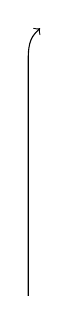
\begin{tikzpicture}[x=0.25cm,y=0.25cm]
\draw[->] (0,0)--(0,12).. controls (0,13) and (0.2,13.2)..(0.6,13.6);
\end{tikzpicture}}

On the other hand the subgroup of
\[
\mathcal M_{\rho,\sigma}(0)\simeq\tau_{\rho,\sigma}\subset B'_0\times T_\rho\times N'_\sigma
\]
which operates trivially on $SG$, is \inserted{the intersection of $\tau_{\rho,\sigma}$ with} $(\deleted{\unsure{\mu_2}}\inserted{1}\times T_\rho\times N'_\sigma)$, for $B'_0$ operates \unsure{trivially} \deleted{$\mu_2\unsure{\subset}B'_0$} (since
\[
(46)\qquad B'_0\cap\underbrace{\mu_2}_{\substack{\text{center of}\\SG}}=\{1\}
\]
. It is therefore the subgroup of the
\[
(47)\qquad
\left\{\left(1,\underset{\in\,\Gamma T_\rho}{\underline a},\underset{\in\,\Gamma N'_\sigma}{\underline b}\right)\mid(\det\underline a)^2=1,\ \det\underline b=1\right\}
\]

\margin{\unsure{no!}}
\uline{Remains} : determine \uline{the center of} $\tau_{\rho,\sigma}$, extension of $\mu_2\times\mu_2$ by $\tau^0_{\rho,\sigma}\simeq\mathcal G^*_{\rho,\sigma}(0)^0\subset T_0^0\times T_\rho\times\deleted{\unsure{N'_\sigma}}\inserted{T_\sigma}$. Since $\tau^0_{\rho,\sigma}$ is commutative, it suffices to determine the action of $\mu_2\times\mu_2$ on $\tau^0_{\rho,\sigma}$, and to determine its subgroup of invariants.
\margin{This will give at least the intersection of the center \unsure{with} $\tau^0_{\rho,\sigma}$.}
\margin{408}

\scanpage{410}
\mspage{506}

Let us note that we have
\[
\tau_{\rho,\sigma}=S\mathcal G^*_{\rho,\sigma}(0)\subset\mathcal G^*_{\rho,\sigma}(0)\simeq T_0\times T_\rho\times N'_\sigma
\]
and we have a homomorphism of exact sequences

\begin{samepage}
\noindent$(48)$\quad
\diagram{\begin{tikzcd}[ampersand replacement=\&,column sep=large,row sep=large]
1\arrow[r]\&\tau^0_{\rho,\sigma}\arrow[r]\arrow[d,hook]
\&\tau_{\rho,\sigma}\arrow[r,"{(\underline u,\underline a,\underline b)\mapsto(\varepsilon(\underline b),\det\underline a/\det(\underline u))}"]\arrow[d,hook]
\&\mu_2\times\mu_2\arrow[r]\arrow[d,"{\substack{\text{first}\\\text{projection}}}"]\&1\\
1\arrow[r]\&\unsure{T_0}\times T_\rho\times\deleted{\unsure{N'_\sigma}}\inserted{T_\sigma}\arrow[r]
\&T_0\times T_\rho\times N'_\sigma\arrow[r]\&\mu_2\arrow[r]\&1
\end{tikzcd}}
\end{samepage},

which shows that the action of $\mu_2\times\mu_2$ on \deleted{$\unsure{\tau}$} $\tau^0_{\rho,\sigma}$ takes place through the projection of $\mu_2\times\mu_2$ onto its first factor, and this by the operation of the latter on $T_0\times T_\rho\times T_\sigma$ which operates trivially on $T_0\times T_\rho$, and which on $T_\sigma$ is the canonical operation of $\mu_2$ on $T_\sigma$, $\sigma\mapsto\varepsilon\sigma$, whose invariants are reduced to the scalars $\mathbb G_m$. \deleted{Thus we find} \inserted{This reasoning} shows, more generally, that the \unsure{trace} \inserted{of the center of $\tau_{\rho,\sigma}$} on the subgroup $\tau'_{\rho,\sigma}\subset\tau_{\rho,\sigma}$ kernel of

\diagram{\begin{tikzcd}[ampersand replacement=\&,column sep=large]
\tau_{\rho,\sigma}\arrow[r]\&\mu_2\times\mu_2\arrow[r,"{\text{1\textsuperscript{st} projection}}"]\&\mu_2\\
(\underline u,\underline a,\underline b)\arrow[rr,mapsto]\&\&\varepsilon(\underline b)
\end{tikzcd}}

is also the trace, on this subgroup, of $T_0\times T_\rho\times\mathbb G_m$. Moreover, since $\mu_2$ operates \uline{faithfully} on $T_\sigma$ via $\sigma\mapsto\varepsilon\sigma$, we see \deleted{that} at once that it also operates faithfully on $\tau'_{\rho,\sigma}$ (which indeed maps \uline{\unsure{epimorphically}} onto $T_\sigma$ !) so we have

\diagram{\begin{tikzcd}[ampersand replacement=\&,column sep=large]
\uline{\mathrm{Centre}}(\tau_{\rho,\sigma})\subset\tau'_{\rho,\sigma}=\operatorname{Ker}\bigl(\tau_{\rho,\sigma}
\arrow[r,"{(\underline u,\underline a,\underline b)\mapsto\varepsilon(\underline b)}"]\&\mu_2\bigr)
\end{tikzcd}}
\margin{409}

\scanpage{411}

Thus in summary
\[
(49)\quad
\left\{
\begin{array}{l}
\uline{\mathrm{Centre}}(\mathcal G^*_{\rho,\sigma}(0))=T_0\times T_\rho\times\mathbb G_m\\[5pt]
\uline{\mathrm{Centre}}\left(\underset{S\mathcal G^*_{\rho,\sigma}(0)}{\underline{\tau_{\rho,\sigma}}}\right)
=\deleted{\unsure{\mathrm{Centre}}}(T_0\times T_\rho\times\mathbb G_m)\cap\tau_{\rho,\sigma}\\[7pt]
\hspace{7em}=\left\{\left(
\underset{\substack{\in\Gamma T_0\\\simeq\Gamma\mathbb G_m}}{\underline u},
\underset{\in\Gamma T_\rho}{\underline a},
\underset{\in\Gamma\mathbb G_m}{\unsure{\lambda}}
\right)\mid u=\lambda^2,\ \deleted{\unsure{\underline a}}\inserted{\det\underline a}=\varepsilon'\unsure{\lambda^2},\ \varepsilon'^2=1\right\}
\end{array}\right.
\]

The subgroup of the center which operates \unsure{trivially} on $SG$ is thus, by (47), given by the additional restriction $u=1$, it thus identifies with \deleted{$\mu_2\times\mu_2$}
\[
(50)\quad
\left\{
\begin{array}{l}
1\times\unsure{ST'_\rho}\times\mu_2\subset\tau^{\unsure{a|0}}_{\rho,\sigma}\subset T_0\times T_\rho\times\unsure{N'_\sigma}\\[5pt]
\text{where }\unsure{ST'_\rho}\subset T_\rho\\[3pt]
\hspace{3em}\Vert\ \{\underline a\mid(\det\underline a]^2=1\}
\end{array}\right.
\]

Thus
\[
(51)\quad
\deleted{\uline{\mathrm{Centr}}(\mathcal M_{\rho,\sigma})\simeq
\left(\underset{\in T_0}{1}\times\unsure{ST'_\rho}\times\underset{\in T_\sigma}{\mu_2}\right)\times\underset{\in SG}{\mu_2}}
\]
\margin{\uline{false} the center is larger,}

The group of integral points of this \deleted{center}\inserted{group}, in the modular case, is reduced:
\[
(52)\quad
\left\{
\begin{array}{l}
\mathbb Z/6\mathbb Z\times\mathbb Z/2\mathbb Z\times\mathbb Z/2\mathbb Z\\[4pt]
\simeq\mathbb Z/3\mathbb Z\times(\mathbb Z/2\mathbb Z\times\mathbb Z/2\mathbb Z\times\mathbb Z/2\mathbb Z),
\end{array}\right.
\]
\deleted{\unsure{Group of}}
\margin{\uline{N.B.} This group is in fact contained in $\mathcal M^0_{\rho,\sigma}(\mathbb Z)$.}

product of a cyclic group of order $3$ (naturally generated by $-\rho$) with a group $(\mathbb Z/2\mathbb Z)^3$, which is none other than the group $\Sigma$ already in (\uline{IX}).

More interesting would probably be the
\margin{410}

\scanpage{412}
\mspage{507}

center of $\mathcal{M}_{\rho,\sigma}^{\circ}$, which will thus be the direct product of the center \inserted{$\mu_2$} of $SG$ (on which the \inserted{\uline{commutative}} group $\mathcal{M}_{\rho,\sigma}^{\circ}(0)\simeq\tau_{\rho,\sigma}^{\circ}$ operates \unsure{trivially}) with the subgroup of $\tau_{\rho,\sigma}^{\circ}\subset T_0\times T_\rho\times T_\sigma$ which operates \unsure{trivially} on $SG$, namely \deleted{$\unsure{\tau_{\rho,\sigma}}$}

\margin{\uline{false}}

\[
\begin{aligned}
\tau_{\rho,\sigma}^{\circ}\cap 1\times T_\rho\times\unsure{T_\sigma}
 &=\{(1,\uline{a},\uline{b})\mid\det\uline{b}=1,\,
 \deleted{(}\det\uline{a}\deleted{)^{\unsure{2}}}=1\}\\
 &\simeq ST_\rho\times ST.
\end{aligned}
\]
\margin{(and not just $(\det a)^2=1$, since we are in $\tau_{\rho,\sigma}^{\circ}$}

Thus

\unsure{We}
\deleted{\diagram{\[\begin{array}{rcl}
(53)\quad\uline{\mathrm{Centre}}(\mathcal{M}_{\rho,\sigma}^{\circ})
 &=&(1\times ST_\rho\times ST_\sigma)\times\mu_2\quad,\\
 &&\hfill\cap\qquad\\[-2pt]
 &&\hfill SG\qquad
\end{array}\]}}

\margin{\uline{false} ! Center \unsure{is} of dimension 3}

thus in the modular case we have

\deleted{\diagram{\[\begin{array}{rclccccccc}
(\unsure{54|14})\quad\uline{\mathrm{Centre}}(\mathcal{M}_{\rho,\sigma}^{\circ})(\mathbb Z)
 &\simeq&1&\times&\mathbb Z/6\mathbb Z&\times&\mathbb Z/4\mathbb Z&\times&\mathbb Z/2\mathbb Z\\
 &&&&\Vert&&\Vert&&\Vert\\
 &&&&\Gamma(ST_\rho)&&\Gamma(ST_\sigma)&&\Gamma\mu_2\subset\Gamma(SG)
\end{array}\]}}

\deleted{which is only twice as large as \deleted{$\unsure{\mathcal{M}_{\rho,\sigma}}$} the group of integral points of the center of $\mathcal{M}_{\rho,\sigma}$. \deleted{(\unsure{although the latter}}}

\deleted{\uline{Remark.} The identity component of the center of $\mathcal{M}_{\rho,\sigma}^{\circ}$ is of course $ST_\rho\times ST_\sigma$, as was suggested by the \unsure{dévissage|discussion} of the theorem on page $501'$.}

\margin{411}

\scanpage{413}
\mspage{508}

\uline{$\overline{\mathrm{XI}}$}\quad\uline{Recapitulation on the group} $\mathcal{M}_{\rho,\sigma}$.

\margin{\uline{Preliminaries}}

\textcircled{$1^\circ$} Given, over a scheme $S$, a form $G$ of $\mathrm{Gl}(2)$, hence forms $SG$, $PG$ of $\mathrm{Sl}(2)$, $\unsure{\mathrm{GP}(1)|\mathrm{PGl}(1)}$, and two sections $\widetilde\rho,\widetilde\sigma$ of $PG$, and a \unsure{1-parameter} \deleted{\unsure{unipotent|multiplicative}} additive \unsure{bordered|based} subgroup
\diagram{\begin{tikzcd}[ampersand replacement=\&,column sep=large]
\widetilde{\uline{\varepsilon}}_0:\ G_a \arrow[r,hook] \& PG
\end{tikzcd}}
\inserted{$\unsure{\varepsilon_0|G_a}$}
(which amounts to the same thing, a \deleted{\unsure{of}} regular unipotent section \unsure{of} $\varepsilon_0$ of $G$, or a regular nilpotent section $N_0$ in the form $\mathcal M$ of $\mathrm{M}_2(\mathcal O_S)$ associated to $G$) --- satisfying the conditions
\[
\begin{aligned}
(1)\quad &\widetilde\sigma^{-1}\widetilde\rho
  =\widetilde{\uline{\varepsilon}}_0(1),\qquad
  \widetilde{\uline{\varepsilon}}_0\text{ and }
  \widetilde{\uline{\varepsilon}}_1
  =\rho\bigl(\widetilde{\uline{\varepsilon}}_0\bigr)
  \bigl(=\sigma\bigl(\widetilde{\uline{\varepsilon}}_0\bigr)\bigr)
  \text{ are}\\
 &\hspace{10em}\text{independent on each fiber}\\[4pt]
(2)\quad &\mathrm{Tr}\,\sigma=0\qquad
 \text{if }\sigma\text{ is a local lifting of }\widetilde\sigma,
\end{aligned}
\]

We define \uline{canonical} liftings $\rho$, $\sigma$ of $\widetilde\rho,\widetilde\sigma$ to $G$, \deleted{\unsure{satisfy}} by the conditions
\[
(3)\quad\deleted{\unsure{\sigma\rho}}
\left\{\begin{array}{ll}
 \varepsilon_0=-\sigma^{-1}\rho
 &\text{i.e. }\varepsilon_1=-\rho\sigma^{-1}\\
 \mathrm{Tr}(\rho+\sigma)=1
 &\text{i.e. }\mathrm{Tr}\,\rho=1,
\end{array}\right.
\]
and the constructions which follow make sense.

We construct a \unsure{pinning}
\diagram{\begin{tikzcd}[ampersand replacement=\&,column sep=large]
\deleted{(\unsure{4})}\ (5)\quad\deleted{\unsure{\tau_{\rho,\sigma}}=}\ \mathrm{Gl}(2)
 \arrow[r,"\sim"] \& G
\end{tikzcd}}
by the condition that $\varepsilon_1$ take the form
\[
(6)\qquad\varepsilon_1
 =\begin{pmatrix}1&0\\1&1\end{pmatrix}
\]
whence
\[
(7)\quad\left\{\begin{array}{l}
\displaystyle\rho=\begin{pmatrix}0&1\\\unsure{v|\upsilon}&1\end{pmatrix},\qquad
 \sigma=\begin{pmatrix}0&-1\\-\unsure{v|\upsilon}&0\end{pmatrix}
 \qquad(\unsure{v|\upsilon}\in\Gamma G_m\\[6pt]
\det\rho=\det\sigma=-\unsure{v|\upsilon}
\end{array}\right.
\]
\[
(8)\qquad\varepsilon_0
 =\begin{pmatrix}1&1/\unsure{v|\upsilon}\\0&1\end{pmatrix},
\]

\margin{412}

\scanpage{414}

we consider the subgroups
\[
(9)\quad\left\{\begin{array}{ll}
 L_0=\{\uline{\varepsilon}_0(\lambda)\}
   =\left\{\begin{pmatrix}1&\lambda\\0&1\end{pmatrix}\right\}
 & (\lambda\in\Gamma G_a)\\[7pt]
 L_1=\sigma(L_0)=\rho(L_0)
   =\{\uline{\varepsilon}_1(\lambda)\}
   =\left\{\begin{pmatrix}1&0\\\lambda&1\end{pmatrix}\right\}
 & \backslash\;\unsure{\text{id}}\\[7pt]
 B'_0=\left\{\begin{pmatrix}\mu&\lambda\\0&1\end{pmatrix}
       \mid\mu\in\Gamma G_m,\,\lambda\in\Gamma G_a\right\} &\\[7pt]
 T_0=\left\{\begin{pmatrix}\mu&0\\0&1\end{pmatrix}
       \mid\mu\in\Gamma G_m\right\} &
\end{array}\right.
\]
whence
\[
(10)\qquad B'_0=T_0.L_0\qquad\text{($\frac12$-direct product)}
\]
\margin{\unsure{---}}

and we have isomorphisms
\diagram{\[
(11)\quad\left\{\begin{gathered}
\begin{tikzcd}[ampersand replacement=\&,column sep=large,row sep=large]
\uline{\varepsilon}_0:\ G_a \arrow[r,"\sim"] \& L_0
 \&\lambda\arrow[r] \&\varepsilon_0(\lambda)
      =\begin{pmatrix}1&\lambda/\unsure{v|\upsilon}\\0&1\end{pmatrix}\\
\uline{\varepsilon}_1:\ G_a \arrow[r,"\sim"] \& L_1
 \&\lambda\arrow[r] \&\varepsilon_1(\lambda)
      =\begin{pmatrix}1&0\\\lambda&1\end{pmatrix}
\end{tikzcd}\\[5pt]
\text{thus }\uline{\varepsilon}_1(\lambda)
  =\rho\unsure{(\,|\{\,}\varepsilon_0(\lambda))
  =\sigma(\varepsilon_0(\lambda)).
\end{gathered}\right.
\]}

We \deleted{set} consider
\[
(12)\quad\deleted{\unsure{\mathcal{G}_{\rho,\sigma}}}
\left\{\begin{aligned}
 T_\rho&=\text{scheme of units of }\mathcal A_\rho
  =\uline{\mathcal O}_S+\uline{\mathcal O}_S\rho\\
 &\hspace{17em}\simeq\uline{\mathcal O}_S[X]/(X^2-X-\unsure{v|\upsilon})\\
 &\deleted{\text{\unsure{of}}\ \uline{\mathcal O}_S}\\
 T_\sigma&=\text{scheme of units of }\mathcal A_\sigma
  =\uline{\mathcal O}_S+\uline{\mathcal O}_S\sigma\\
 &\hspace{17em}\simeq\uline{\mathcal O}_S[Y]/(Y^2-\unsure{v|\upsilon})
\end{aligned}\right.
\]
\diagram{\[\begin{array}{rcl}
(13)\quad &N'_\sigma&=\{g\in\Gamma G\mid g(\sigma)=\varepsilon\sigma,\ \varepsilon^2=1\}\\
 &\cap&\\[-2pt]
 &G&
\end{array}\]}
whence
\diagram{\begin{tikzcd}[ampersand replacement=\&,column sep=large]
(14)\quad 1\arrow[r] \&T_\sigma\arrow[r] \&N'_\sigma\arrow[r,"\varepsilon_\sigma"] \&\mu_2\arrow[r] \&1.
\end{tikzcd}}

We set
\[
(15)\quad\left\{\begin{aligned}
 \mathcal{G}_{\rho,\sigma}&=B'_0\times T_\rho\times T_\sigma\\[4pt]
 \mathcal{G}_{\rho,\sigma}^{*}&=B'_0\times T_\rho\times N'_\sigma.
\end{aligned}\right.
\]

\margin{413}

\scanpage{415}
\mspage{509}

\margin{$\begin{gathered}
 \mathcal M_{\rho,\sigma}[0],\ \mathcal M_{\rho,\sigma}(0)\,,\\
 \unsure{\tau_{\rho,\sigma}|\mathcal G_{\rho,\sigma}},\ \tau_{\rho,\sigma}^{\circ}\,,\\
 \mathcal M_{\rho,\sigma},\ \widetilde{\mathcal G}_{\rho,\sigma}^{+}\quad
   \deleted{\unsure{\mathcal M_{\rho,\sigma}^{\circ}}}\\
 \tau_{\rho,\sigma}^{\circ+}
\end{gathered}$}

\textcircled{$2^\circ$} We introduce
\[
\begin{aligned}
(16)\quad \mathcal M_{\rho,\sigma}[0]
 &\subset \unsure{\mathcal B_{\rho,\sigma}^{*}|\mathcal G_{\rho,\sigma}^{*}}
   =B'_0\times T_\rho\times N'_\sigma\\
 &\mathrel{\mathop{=}\limits^{\mathrm{dfn}}}
 \{(\uline u,\uline a,\uline b)\mid
   \det\uline u=\det\uline b=\varepsilon'\det\uline a,\
   \varepsilon'{}^2=1\}
\end{aligned}
\]
\[
(17)\qquad \mathcal M_{\rho,\sigma}(0)\subset\mathcal M_{\rho,\sigma}[0]
 \qquad\text{defined by }\uline u=1\quad\text{i.e.}
\]
\[
 \mathcal M_{\rho,\sigma}(0)=\mathcal M_{\rho,\sigma}[0]
   \cap(T_0\times T_\rho\times N'_\sigma)
 \qquad\text{in }\mathcal G_{\rho,\sigma}^{*}.
\]
\diagram{\begin{tikzcd}[ampersand replacement=\&,column sep=large,row sep=small]
(18)\quad L_0\arrow[r,hook] \&\mathcal M_{\rho,\sigma}[0]\\
\lambda\arrow[r,mapsto] \&(\lambda,1,1)
\end{tikzcd}}
thus we have
\[
(19)\qquad \mathcal M_{\rho,\sigma}[0]\simeq
  \mathcal M_{\rho,\sigma}\unsure{[0)|(0)}\, .\, L_0
 \qquad\text{product }\tfrac12\text{-direct}
\]

We have a homomorphism
\diagram{\begin{tikzcd}[ampersand replacement=\&,column sep=huge]
(20)\quad\unsure{\dot{\mathcal M}|\mathcal M}_{\rho,\sigma}[0]\arrow[r]
 \&G_m\times\mu_2\times\mu_2
\end{tikzcd}}
\[
 \text{denoted }\{g\mapsto\chi(g),\varepsilon_2(g),\varepsilon_3(g)
\]
for $g=(\uline u,\uline a,\uline b)$ we have
\[
\begin{aligned}
 \chi(g)&=\det\uline u=\det\uline b\\
 \varepsilon_2(g)&=\varepsilon_\sigma(b)\qquad\text{(cf. (13)(14)}\\
 \varepsilon_3(g)&=\det(\uline a)/\det\uline b\\
 &\text{i.e. }\left\{\begin{array}{l}
    \det a=\varepsilon_3\mu\\
    \text{where }\mu=\chi(g)
  \end{array}\right.
\end{aligned}
\]
trivial on $L_0$ (thus factoring through the quotient). We also set
\[
(21)\qquad\tau_{\rho,\sigma}\simeq\mathcal M_{\rho,\sigma}[0]/L_0
 \qquad\text{\unsure{where}}
\]
\margin{This notation is not at all adequate (\unsure{wrongly inspired} by $\tau_{g,\unsure{\nu|r}}$) \unsure{the sequel shows} (and what precedes already showed) that the notation $\Gamma_{\rho,\sigma}$ would be suitable, inspired by $\Gamma_{g,\nu}$ and $\Gamma_{0,3}$.}

\unsure{and} the composite
\diagram{\begin{tikzcd}[ampersand replacement=\&,column sep=large]
(22)\quad\mathcal M_{\rho,\sigma}(0)\arrow[r,hook]
 \&\mathcal M_{\rho,\sigma}[0]\arrow[r] \&\tau_{\rho,\sigma}
\end{tikzcd}}
is an \uline{isomorphism}, whence we have
\diagram{\begin{tikzcd}[ampersand replacement=\&,column sep=large]
(23)\quad\unsure{\mathcal M|\mathcal G}_{\rho,\sigma}(0)
 \simeq\unsure{\tau_{\rho,\sigma}|\tau_{\rho,\sigma}'}\arrow[r,hook]
 \&T_0\times T_\rho\times N'_\sigma
\end{tikzcd}}

\margin{414}
